\documentclass[8pt]{beamer}
\usepackage[dutch]{babel}
\usepackage{lmodern}
\usetheme{Madrid}

\usepackage{url}
\usepackage{natbib}

\usepackage{amsmath}
\usepackage{amsopn}
\usepackage{amsthm}

\DeclareMathOperator*{\argmin}{arg\,min}
\DeclareMathOperator*{\argmax}{arg\,max}


% Change base colour beamer@blendedblue (originally RGB: 0.2,0.2,0.7)
\colorlet{beamer@blendedblue}{green!40!black}

\title{\textbf{Co}ntext as \textbf{Li}nguistic \textbf{Bri}dges}
\author{Maarten van Gompel}
\date{\vspace{-10ex} {24 maart 2020}}
\usepackage{graphicx}
\usepackage{placeins}



\def\raccoon{
\makebox[\linewidth][c]{\includegraphics[width=70pt]{/home/proycon/Pictures/All/raccoon.pdf}\FloatBarrier}
}
\def\smallraccoon{
\makebox[\linewidth][c]{\includegraphics[width=30pt]{/home/proycon/Pictures/All/raccoon.pdf}\FloatBarrier}
}

\begin{document}

\begin{frame}
	\titlepage
    \makebox[\linewidth][c]{\includegraphics[width=6cm]{../thesis/drawing-eps-converted-to.pdf}\FloatBarrier}
\end{frame}

\section{Inleiding}

\begin{frame}{Inleiding}

	\begin{block}{Context}
        \begin{itemize}
            %Algemene intuitie
            \item \textbf{Intuïtie:} \emph{``Context speelt een belangrijke rol in taal''}
            \item Betekenis van woorden, zinsneden, zinnen etc... is afhankelijk van de context waarin ze verschijnen.
            \item Context helpt eventuele ambiguïteit in betekenis op te lossen
        \end{itemize}
	\end{block}

    \begin{block}{Voorbeeld: een woord}
        {\Large\textbf{``bank''}}

        Volgens van Dale:
        \begin{enumerate}
            \item zitmeubel voor meer dan één persoon
            \item verkooptafel: toonbank
            \item werktafel: draaibank
            \item door de natuur gevormde ondiepte
            \item instelling die gelden beheert en uitleent
            \item (bij kansspelen) inzet van de hoofdspeler tegen alle andere samen
            \item centrale bewaar- en uitwisselingsplaats; = opslagplaats: bloedbank, vacaturebank
        \end{enumerate}
    \end{block}
\end{frame}

\begin{frame}

    \begin{block}{Voorbeeld 1: een woord in context}
        {\Large\textbf{``bank''}}
        \begin{itemize}
            \item \emph{``De \textbf{bank} heeft al mijn geld verloren.''}
            \item \emph{``De hond mag op de \textbf{bank} liggen.''}
        \end{itemize}
    \end{block}

    \begin{block}{Word Sense Disambiguation}
        \begin{itemize}
            \item Context helpt bij het vinden van de betekenis
            \item Het automatisch disambigueren van de juiste betekenis van een woord heet \textbf{Word Sense Disambiguation}.
        \end{itemize}
    \end{block}
\end{frame}


\begin{frame}

    \begin{block}{Voorbeeld 1: Een woord in context}
        {\Large\textbf{``bank''}}
        \begin{itemize}
            \item \emph{``De \textbf{bank} heeft al mijn geld verloren.''}
            \begin{itemize}
                \item<2-> \emph{``La \textbf{banque} à perdu tout mon argent.''}
            \end{itemize}
            \item \emph{``De hond mag op de \textbf{bank} liggen.''}
            \begin{itemize}
                \item<2-> \emph{``Le chien peut se mettre sur \textbf{le canapé}.''}
            \end{itemize}
        \end{itemize}
    \end{block}

    \begin{block}{Betekenis en Vertalingen}
        \begin{itemize}
            \item Het vinden van de juiste betekenis is belangrijk bij vertalen
            \item Een woord kan anders vertalen naar gelang de betekenis
        \end{itemize}
    \end{block}


\end{frame}

\begin{frame}

    \begin{block}{Voorbeeld 2: Een woord in context}
        {\Large\textbf{``tempo''}} (portugees)
        \begin{itemize}
            \item \emph{``Faz bom \textbf{tempo} hoje.``}
            \begin{itemize}
                \item<2-> \emph{``Het is lekker \textbf{weer} vandaag``}
            \end{itemize}
            \item \emph{``Ele tem \textbf{tempo} para mim.''}
            \begin{itemize}
                \item<2-> \emph{``Hij heeft \textbf{tijd} voor mij.``}
            \end{itemize}
        \end{itemize}
    \end{block}

\end{frame}

\begin{frame}

	\begin{block}{Onderzoek}
        \begin{itemize}
            \item De rol van contextinformatie in automatische vertaling
            \item \textbf{Hoofdvraag:} In hoeverre kunnen we automatische vertaling verbeteren door contextinformatie uit de brontaal mee te nemen?
            \item Empirische studie: Schrijven van softwaresystemen, trainen op trainingsdata, testen op testdata,
                vergelijken met anderen, conclusies afleiden
        \end{itemize}
	\end{block}

\end{frame}


\section{Word Sense Disambiguation (hfd 3)}

\begin{frame}{Word Sense Disambiguation}

	\begin{block}{SemEval taken}
        \begin{itemize}
            %in deze eerste fase van het onderzoek..
            \item Vertalen van gemarkeerde fragmenten in context
            %gecontroleerde versimpelde setting, goed om onze hypothese uit te testen
            \item Drie SemEval taken:
            \begin{itemize}
                \item SemEval 2010: Cross Lingual Lexical Substitution (Engels naar Spaans) \citep{CLLS}
                \begin{itemize}
                    \item<2-> (Alleen zelfstandige naamwoorden, lemmas als vertaling)
                \end{itemize}
                \item SemEval 2010: Cross Lingual Word Sense Disambiguation (Engels naar Nederlands/Spaans) \citep{WSD}
                \begin{itemize}
                    \item<2-> (Ook werkwoorden, adjectieven/bijwoorden, lemmas als vertaling)
                \end{itemize}
                \item SemEval 2013: Cross Lingual Word Sense Disambiguation (Engels naar
                    Nederlands/Spaans/Frans/Duits/Italiaans) \citep{CLWSD2013TASKPAPER}
                \begin{itemize}
                    \item<2-> (Alleen zelfstandige naamwoorden, lemmas als vertaling)
                \end{itemize}
            \end{itemize}
        \end{itemize}
	\end{block}

\end{frame}


\begin{frame}
    \begin{block}{Het WSD systeem: Hoe kunnen we context gebruiken voor vertaling?}
        \begin{itemize}
            \item \textbf{Memory-based machine learning}: Een classifier-gebaseerd systeem (Timbl, IB1)
            \item We leren op basis van trainingsdata hoe een woord met bepaalde \textbf{context-features} vertaald
                wordt:
            %voor (pos_s,lemma_s)
            \begin{itemize}
                \item Lokale contextinformatie (woordvorm): $x$ woorden links, $y$ woorden rechts
                \item Linguïstisch verrijkte lokale contextinformatie (PoS$+$lemma)
                \item Globale contextinformatie (woordvorm) \footnotesize{(binary bag of word features)}
            \end{itemize}
            \item \textbf{Word/classifier experts:} We bouwen een classifier voor elk woord (PoS,lemma) dat vertaald
                moet worden
        \end{itemize}
    \end{block}

\end{frame}


\begin{frame}
    \begin{block}{Deelvragen \& Resultaten}
        \begin{enumerate}
            \item Welke informatie draagt het meeste bij tot een juiste vertaling?
            \begin{itemize}
                \item Linguïstisch-geïnformeerd of niet?
                \begin{itemize}
                    \item<2-> Lemmas features helpen, PoS juist niet
                \end{itemize}
                \item Lokale en/of globale features?
                \begin{itemize}
                    \item<2-> In eerste instantie (WSD1) wat positief effect van globale features, maar later (WSD2) niet
                \end{itemize}
                \item Contextgrootte?
                \begin{itemize}
                    \item<2-> Kleine contextgrootte werkt het best (1 links, 1 rechts)
                \end{itemize}
            \end{itemize}
            \item Welke optimalisatietechnieken kunnen we toepassen?
            \begin{itemize}
                \item<2-> Arbiter Voting (WSD1, 2010)
                \item<2-> Automatische feature selectie (WSD2, 2013)
                \item<2-> Classifier parameteroptimalisatie (WSD2, 2013)
            \end{itemize}
        \end{enumerate}
    \end{block}
    \begin{block}{Competitie Resultaten}
        \begin{itemize}
            \item<2-> Winnende scores in de Cross Lingual WSD taak (2010), later ook een aantal winnende scores in 2013
        \end{itemize}
    \end{block}
\end{frame}

\section{Vertalen van L1 fragmenten in een L2 context}


\begin{frame}{Vertalen van L1 fragmenten in een L2 context (hfd 4-6)}
    \begin{block}{Een nieuwe insteek}
        \begin{enumerate}
            \item \textbf{codewisseling/code switching}: het overspringen tussen twee talen
            \item het gebruiken van korte fragmenten van de ene taal in een anderstalige context (bv. zin)
            \item kunnen we zulke vertalingen automatiseren en de anderstalige context daarbij gebruiken?
        \end{enumerate}
    \end{block}

    \begin{block}{Voorbeeld 1: Codewisseling met één woord}
        L1 = Nederlands, L2 = Duits
        \begin{enumerate}
            \item ''Alles was er sagt ist \textbf{altijd} falsch''
            \item ''Alles was er sagt is \textbf{immer} falsch''
        \end{enumerate}
    \end{block}

    \begin{block}{Voorbeeld 2: Codewisseling met langer fragment}
        L1 = Nederlands, L2 = Duits
        \begin{enumerate}
            \item ''Alles \textbf{wat hij zegt} ist immer falsch''
            \item ''Alles \textbf{was er sagt} is immer falsch''
        \end{enumerate}
    \end{block}
\end{frame}

\begin{frame}
    \begin{block}{Opzet}
        \begin{itemize}
            \item Zit er waarde in dit idee?
            \begin{itemize}
                \item Ja, denk aan vertaalhulp systemen
            \end{itemize}
            \item Kunnen we dit net als voorheen met classifiers oplossen? $\rightarrow$
                \textbf{pilot study} (hfd 4)
            \begin{itemize}
                \item<2-> Ja
                \item<2-> Maar; we hebben geen echte representatieve data om op te testen
            \end{itemize}
        \item<3-> Testdata samenstellen en daarmee een nieuwe SemEval taak organizeren (hfd 5)
            \begin{itemize}
                \item<3-> 4 taalparen (L1-L2): Engels-Spaans, Engels-Duits, Frans-Engels, Nederlands-Engels
                \item<3-> Handmatige dataverzameling uit verschillende bronnen
                \item<3-> 6 kandidaten doen mee met onze taak
            \end{itemize}
            \item<3-> Hiermee ons eigen systeem \emph{(colibrita)} opnieuw testen en verbeteren (hfd 6)
        \end{itemize}
    \end{block}
\end{frame}

\section{Statistical Machine Translation}

\begin{frame}{Statistical Machine Translation (hfd 6-7)}

    \begin{block}{Van WSD naar SMT}
        Van \textbf{Word Sense Disambiguation} naar (phrase-based) \textbf{Statistical Machine Translation}
        \begin{itemize}
            \item Naar mate we langere fragmenten bezien begeven we ons steeds meer op de het terrein van de SMT
            \item Kunnen SMT technieken ook toegepast worden in het code-switching scenario?
            \begin{itemize}
                \item<2-> Ja, twee deelnemers aan onze taak laten dit duidelijk zien
                \item<2-> Resultaten beter dan pure classifier aanpak
            \end{itemize}
            \item \textbf{Beste van beide werelden?} Kunnen we de expliciete modellering van de classifiers integreren in SMT en heeft dat meerwaarde? (hfd 6,7)
           \begin{itemize}
               \item<2-> We vergelijken classifiers, classifiers geïntegreerd in SMT, en pure SMT
           \end{itemize}

        \end{itemize}
    \end{block}
\end{frame}


\begin{frame}
    \begin{block}{Phrase-based Statistical Machine Translation}
        \begin{itemize}
            \item Een spel van waarschijnlijkheden, vind de meest waarschijnlijke reeks woorden in de doeltaal gegeven
                een reeks woorden in de brontaal.
            \item Twee modellen modelleren dit: \textbf{vertaalmodel} en \textbf{taalmodel}
                {\footnotesize ($\hat{T} = \argmax_T p(T|S) = \argmax_T \frac{p(S|T)p(T)}{p(S)} = \argmax_T p(S|T)p(T)$)
                }
            \item De twee modellen worden getraind op respectievelijk een \textbf{parallel corpus} en een \textbf{monolinguaal corpus}
            \begin{itemize}
                \item Welke woorden komen vaak samen voor? \emph{(word alignment)}
                \item Welke \textbf{frasen} kunnen daaruit geextraheerd worden? \emph{(phrase extraction)} $\rightarrow$
                    \textbf{phrase-translation table}
            \end{itemize}
        \end{itemize}
    \end{block}

	\begin{center}
	 
\includegraphics[width=45.0mm]{../align1.png} 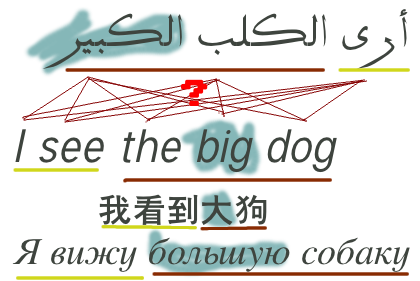
\includegraphics[width=45.0mm]{../align2.png}
	\end{center}

\end{frame}

\begin{frame}
    \begin{block}{Integratie van classifiers in SMT}
        \begin{itemize}
            \item Op welke manieren kunnen we classifiers in SMT integreren?
            \begin{itemize}
                \item \footnotesize{(\emph{classifiertype:} classifier experts vs. monolithisch) , (\emph{weegmethode:} replace vs append)}
                \item<2-> Minimale verschillen met weinig effect in het algemeen, geen eenduidige conclusie te vormen
            \end{itemize}
            \item Heeft data zonder linguïstische verrijking een maarwaarde in deze opstelling?
            \begin{itemize}
                \item<2-> Nee, de \textbf{hoofdconclusie} is dat we expliciet proberen te modelleren wat de bestaande modellen
                    (vertaalmodel + taalmodel) impliciet al goed genoeg dekken. Daar waar contextinformatie uit de
                    brontaal een disambiguerende rol kan spelen, is hij al potentieel beschikbaar in het vertaalmodel.
           \end{itemize}
        \end{itemize}
    \end{block}
\end{frame}

\begin{frame}{Conclusies}
    \begin{block}{Conclusies}
        \begin{enumerate}
            \item Contextinformatie is nuttig voor vertaling (ook met anderstalige context)
            \item We sluiten een lijn van onderzoek
                \citep{Stroppa+07,Rejwanul+11}
                {\footnotesize (de integratie van niet-linguïstische-geinformeerde
                classifier-gebaseerde WSD technieken in (PB)SMT)}
                en concluderen dat deze oplossing geen meerwaarde
                biedt.
                %meer voor de hand ligt het LM verbeteren
            \item We creëren vaak marginale lokale verschillen en concluderen dat een gedegen evaluatie op automatische
                metrieken en bij een gebrek aan meerdere referentievertalingen erg lastig is.
            \item We benadrukken het belang van testen op meerdere datasets, meerdere taalparen, en het doen van
                significantietests om niet te snel conclusies te trekken.
        \end{enumerate}
    \end{block}
\end{frame}

\begin{frame}[allowframebreaks]
        \frametitle{References}
        \bibliographystyle{apalike}
        \bibliography{../thesis/thesis}
\end{frame}

\end{document}

